
\chapter{Analisi dei Requisiti}
In questa fase sono stati individuati i \textbf{requisiti del sistema}, partendo dalle descrizioni di alto livello, ottenute dal committente durante il \textbf{knowledge crunching}. Successivamente si è proceduto con un raffinamento che ha portato alla definizione di requisiti più \textbf{specifici}, \textbf{chiari} e \textbf{strutturati}.
	\section{Requisiti di Business}
	Si definiscono di seguito le aspettative del cliente e i requisiti che il prodotto dovrà soddisfare, espressi con una terminologia ad elevato livello astrattivo.
        \begin{itemize}
            \item Il prodotto dovrà \textbf{diminuire l'intervento umano} necessario per la quotidiana cura degli ospiti (Riempimento ciotola acqua/cibo); la riduzione del lavoro deve essere maggiore o uguale al 30\%.
            \item Il prodotto dovrà consentire di \textbf{diminuire il lavoro su base volontaria}, grazie alla riduzione delle operazioni di cura quotidiana, permettendo ai volontari di concentrarsi solo sulla socializzazione e lo svago dell'animale.
            Diminuisce così l'interferenza al di fuori delle loro mansioni, e migliora la tracciabilità del lavoro svolto, essendo il lavoro volontario incostante e meno affidabile.
            \item Opzionalmente il prodotto dovrà \textbf{fornire un monitoraggio a distanza} degli animali ospitati.
            Questo consentirà al personale incaricato di monitorare parametri come: frequenza cardiaca e temperatura corporea. Verrà diminuito anche l'intervento veterinario, non essendo necessaria la presenza in loco del professionista. La riduzione delle presenze dovrà consentire di diminuire i costi di un valore maggiore o uguale al 10\%.
        \end{itemize}
	
	\section{Requisiti Utente}
	Di seguito vengono riportate le richieste mosse dal cliente in maniera informale evitando termini tecnici, successivamente tali richieste saranno formalizzate per quanto possibile.
	Il prodotto dovrà fornire: 
		\begin{itemize}
            \item l'accesso al sistema da qualunque dispositivo munito di connessione alla rete, anche esterna al canile
            \item prestazioni adeguate alle operazioni richieste (con soglie adeguate caso per caso), come il rilevare se il cane ha bisogno di cibo o acqua 
            \item una restrizione delle funzionalità disponibili in base all'utente
            \item un interfaccia intuitiva, comprensiva di una pagina per l'accesso e un menu principale
            \item uno storico per ogni animale
            \item un accesso rapido e reattivo evitando tempi troppo lunghi per le operazioni
            \item un sistema di sorveglianza semi automatizzato in grado di identificare eventuali anomalie, come cani che escono senza permesso
            \item \textbf{opzionalmente} delle notifiche sullo stato di salute dell'animale al personale
            \item delle notifiche in caso di malfunzionamento del sistema stesso
            \item delle notifiche, nel caso in cui il cibo sia in esaurimento 
        \end{itemize}
        \subsection{User stories}
        Di seguito sono riportate tutte le \textbf{user stories} ritenute utili per lo sviluppo del prodotto.
        \begin{itemize}
            \item Come \textbf{gestore}
            voglio:
            \begin{itemize}
                \item poter visualizzare le i dati relativi all’occupante di una gabbia
                \item voglio poter impostare i dati dell’occupante di una gabbia
                \item poter rimuovere un cane da una gabbia
                \item poter visualizzare i consumi TOTALI del canile
                \item \textit{opzionalmente} poter visualizzare l’umidità e la temperatura ambientale 
                \item poter \textbf{impostare} i dati relativi allo \textbf{stato di salute} di un cane
                \item poter visualizzare i \textbf{consumi di cibo} relativi a un cane in un determinato lasso di tempo
                \item poter visualizzare i \textbf{consumi di acqua} relativi a un cane in un determinato lasso di tempo
            \end{itemize}
            
            \item Come \textbf{responsabile sanitario}
            voglio:
            \begin{itemize}
                \item \textit{opzionalmente} poter \textbf{visualizzare i battiti} di un cane 
                \item  \textit{opzionalmente} ricevere una \textbf{notifica} in caso di rilevazione di \textbf{anomalie} nei \textbf{battiti} o nella di un cane
                \item \textit{opzionalmente} poter \textbf{visualizzare la temperatura corporea} di un cane
                \item \textit{opzionalmente} ricevere una \textbf{notifica} in caso di rilevazione di \textbf{anomalie} nella \textbf{temperatura} corporea di un cane
                 \item \textit{opzionalmente} poter \textbf{impostare} gli intervalli di \textbf{temperatura e battiti} fuori dai quali vi è un’anomalia
                \item poter \textbf{impostare} gli intervalli delle \textbf{quantità di cibo e acqua } assunti, fuori dai quali vi è un’anomalia
                \item ricevere una \textbf{notifica} in caso di \textbf{anomalie} nella quantità di \textbf{acqua} assunta da un cane
                \item ricevere una \textbf{notifica} in caso di \textbf{anomalie} nella quantità di \textbf{cibo} assunto da un cane
                \item poter \textbf{impostare} i dati relativi allo \textbf{stato di salute} di un cane
                \item poter \textbf{impostare la quantità di cibo} da erogare a un cane
                \item poter visualizzare i \textbf{consumi di cibo} relativi a un cane in un determinato lasso di tempo
                \item poter visualizzare i \textbf{consumi di acqua} relativi a un cane in un determinato lasso di tempo
            \end{itemize}
            
            \item Come \textbf{addetto ai  rifornimenti}
            voglio:
            \begin{itemize}
                \item essere notificato se in una gabbia sta per esaurirsi il cibo
                \item ricevere una notifica in caso di malfunzionamento al sistema
                \item poter impostare la quantità di cibo da erogare a tutti i cani di una determinata taglia
                \item poter \textbf{impostare la quantità di cibo} da erogare a un cane
                \item poter visualizzare i \textbf{consumi di cibo} relativi a un cane in un determinato lasso di tempo
                \item poter visualizzare i \textbf{consumi di acqua} relativi a un cane in un determinato lasso di tempo
            \end{itemize}
            
            \item Come \textbf{addetto alla sorveglianza}
            voglio:
            \begin{itemize}
                \item poter visualizzare le immagini acquisite dalla videocamera di sorveglianza
                \item notificato in caso di uscita non autorizzata di un cane
                \item \textit{opzionalmente} essere notificato in caso di rilevazione di suoni forti o anomali
                \item \textit{opzionalmente} poter visualizzare l’umidità e la temperatura ambientale 
            \end{itemize}
        \end{itemize}
        
        Di seguito viene riportato lo schema, sotto-forma di diagramma di Venn, esplicativo delle intersezioni tra le User-Stories e le figure dell'organigramma. 
        %TABELLA CONTEXT MAP
        \begin{figure}[ht]
            \caption{Diagramma di Venn delle User-Stories}
            \centering
            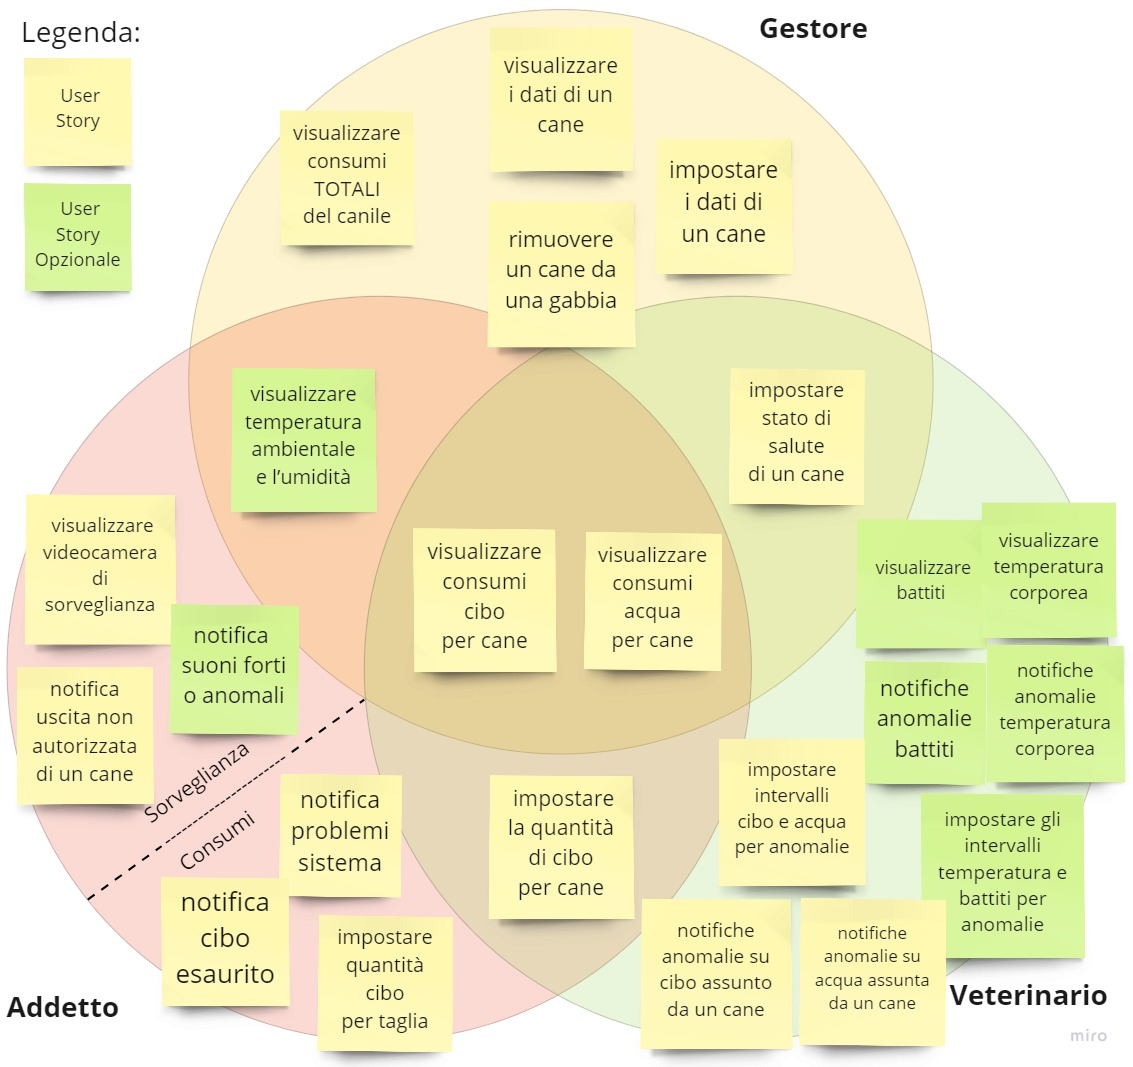
\includegraphics[width=1\textwidth]{Miro/DiagrammaUserStories.jpg}
        \end{figure}
    
	    
	\section{Requisiti Funzionali} %obbligatori, desiderabili e opzionali
	    \subsection{Casi d'uso}
        	 %Diagramma dei casi d'uso
            \begin{figure}[ht]
                \caption{Diagramma dei casi d'uso del sistema, rappresenta le principali azioni effettuate degli attori}
                \centering
               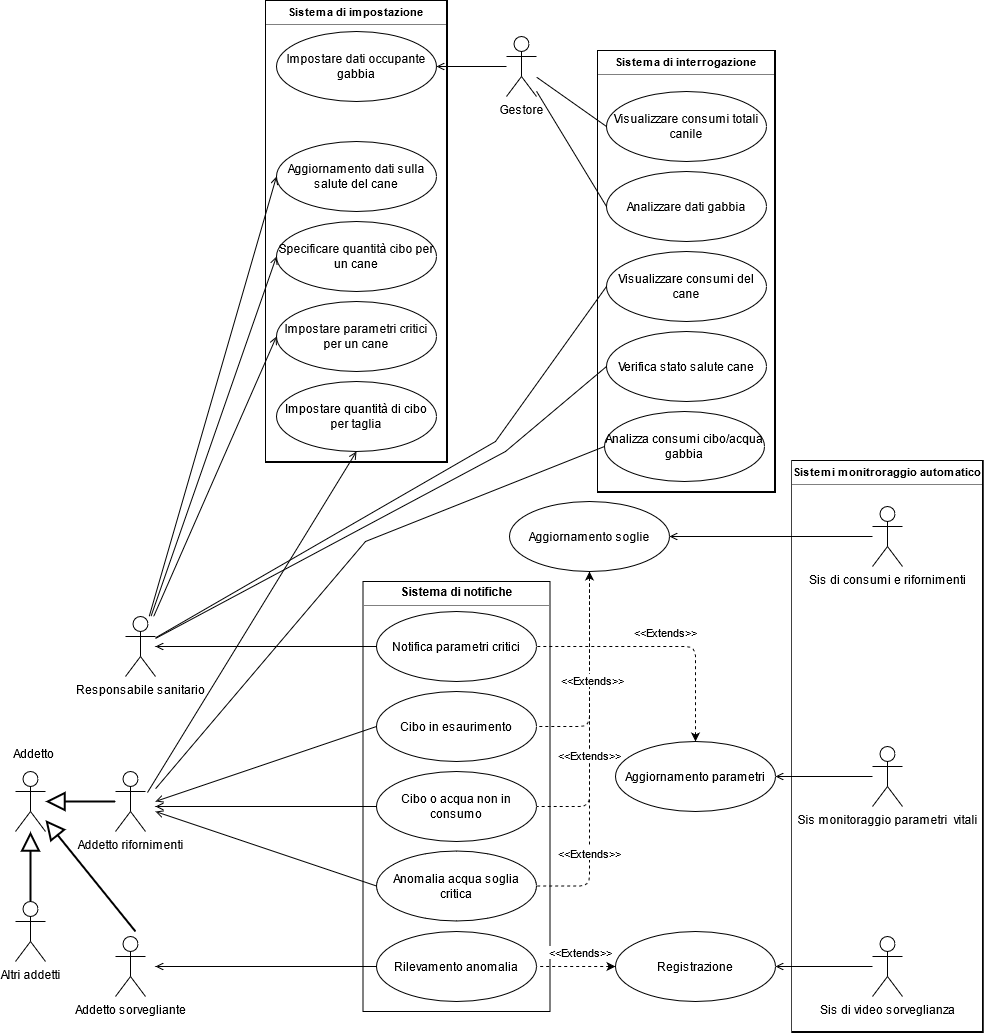
\includegraphics[width=0.9\textwidth]{DrawIo/useCaseWholeSystem.png}
            \end{figure}
            
    	Si elencano i requisiti funzionali per ognuno dei seguenti macro-componenti:
	    \begin{itemize}
            \item Applicativo web 
            \item Applicativo video
            \item Opzionale collare
            \item Strumentazione gabbia
        \end{itemize}
        
    \subsection{Applicativo web}
        L'applicativo web deve consentire ad ogni utente di accedere con una serie di credenziali, e dividere le operazioni consentite in base ai permessi concessi.
        Il sito è suddiviso in tre pagine principali:
        \begin{itemize}
            \item \textbf{pagina di login}
                La pagina iniziale a cui ogni utente deve far riferimento per effettuare l'accesso.
                Sostanzialmente contiene solo gli elementi necessari per effettuare il \textbf{login}, non è prevista una funzione di registrazione autonoma.
            \item \textbf{home gestore}
                Il gestore ha accesso alla pagina di amministrazione, dov'è possibile:
                \begin{itemize}
                    \item registrare un nuovo utente
                    \item eliminare un utente
                    \item visualizzare le statistiche del canile
                \end{itemize}
            \item \textbf{home addetto rifornimenti}
                La schermata deve consentire di:
               \begin{itemize}
                    \item visualizzare le eventuali notifiche
                    \item visualizzare i consumi di un cane
                    \item impostare la quantità di cibo adeguata per taglia di cane
                \end{itemize}
            \item \textbf{home addetto sorveglianza}
                La home del sorvegliante deve fornire:
               \begin{itemize}
                    \item un accesso in diretta alle videocamere disponibili
                    \item deve essere possibile aggiungere o rimuovere una videocamera
                    \item visualizzare le notifiche se presenti
                \end{itemize}
            \item \textbf{home altri addetti}
                In un futuro sviluppo del prodotto è certamente contemplata l'aggiunta di altre mansioni o addetti.
            \item \textbf{responsabile sanitario}
                La pagina deve consentire di:
               \begin{itemize}
                    \item visualizzare lo stato di salute di un cane
                    \item visualizzare i consumi di un cane
                    \item impostare la quantità di cibo per un cane degente o in terapia
                    \item aggiornare lo stato di salute di un cane
                \end{itemize}
        \end{itemize}
        
    Nonostante un addetto possa ricoprire più ruoli, è stato scelto di modellare separatamente ogni mansione, questo consente: un maggiore controllo, rende più chiara la struttura e aiuta il lettore nella comprensione.
    Inoltre l'applicativo consentirà ad un utente di detenere uno o più ruoli, rendendo più agevole l'utilizzo. 
    \subsection{Opzionale: collare}
        Il collare smart deve costantemente inviare aggiornamenti sui parametri vitali dell'animale quali:
            \begin{itemize}
                \item La frequenza cardiaca
                \item La temperatura dell'animale
            \end{itemize}
    \subsection{Strumentazione gabbia}
        La gabbia smart deve:
            \begin{itemize}
                \item monitorare il consumo di cibo e acqua del cane inviando aggiornamenti costanti
                \item rifornire la ciotola di acqua quando troppo bassa
                \item rifornire la ciotola di cibo quando troppo vuota
            \end{itemize}
    \subsection{Strumentazione videosorveglianza}
        La strumentazione deve fornire uno streaming video e audio costante nel tempo. La bidirezionalità è opzionale.
        
	\section{Requisiti non Funzionali}
	Il primo vicolo individuato è quello economico. Il costo del servizio, essendo l'attività non a scopo di lucro e mantenuta grazie all'azione dei volontari, deve essere minimo. Questo è comprensivo dell'istallazione, dei materiali e dei costi di servizio.
	Un secondo vincolo rappresenta la sicurezza, l'eventuale introduzione di strumentazione all'interno del canile non deve rappresentare in alcun modo un pericolo per la salute dell'animale.
	
    Il sistema dovrà rispettare alcuni requisiti non funzionali che ne determineranno la \textbf{qualità}:
        \subsection{Di Sistema}
            \begin{itemize}
            \item \textbf{Reattività}: 
            \begin{itemize}
                \item l'utente non deve percepire \textbf{ritardi} nell'ordine dei secondi tra l'invio di un comando e l'esecuzione dello stesso all'interno della piattaforma. 
                \item le notifiche standard del sistema devono essere mostrate ai relativi utenti con un ritardo complessivo massimo non superiore al minuto.
                \item le notifiche urgenti del sistema, ossia quelle relative a malfunzionamenti gravi o alla salute dell'animale, devono essere mostrate ai relativi utenti con un ritardo complessivo massimo non superiore ai dieci secondi.
            \end{itemize}
            
            \item \textbf{Scalabilità}: L'applicativo deve necessariamente consentire di aumentare o diminuire il numero di animali gestiti. Ciò deve avvenire senza una sensibile ripercussione sulle prestazioni del sistema e un disagio minimo a livello pratico. Per prevenire, inoltre, che la presenza di una connessione cablata limiti la scalabilità del sistema, è desiderabile che non ci siano altri collegamenti al di fuori dell'alimentazione già presente. 
            
            \item \textbf{Fault tolerance}: la \textbf{gestione degli errori} deve essere adeguatamente implementata affinché le interruzioni involontarie non danneggino innanzitutto la salute degli animali.
            Eventuali malfunzionamenti di apparecchiature o sensoristica all'interno del canile non devono pregiudicare il funzionamento complessivo dell'applicativo, ma al massimo della singola unità logica. 
    \end{itemize}
        
    \subsection{Della Sensoristica}
    \begin{itemize}
        \item \textbf{Precisione}:
            \begin{itemize}
                \item \textbf{Bilancia} lo scostamento massimo tra più misure deve essere inferiore o uguale a 10 grammi.
                \item \textbf{Temperatura} lo scostamento massimo tra più misure deve essere inferiore o uguale a 2 gradi.
                \item \textbf{Umidità} lo scostamento massimo tra più misure deve essere inferiore o uguale a 5\%.
                \item \textbf{Livello acqua} lo scostamento massimo tra più misure deve essere inferiore o uguale a 1 centimetro.
                \item \textbf{Frequenza cardiaca} lo scarto tra misure sulla stessa frequenza deve essere al massimo 10 battiti.
            \end{itemize}
        \item \textbf{Risoluzione}:
            \begin{itemize}
                \item \textbf{Bilancia} il range di misura, partendo da vuota, deve riuscire a comprendere almeno un Kg.
                \item \textbf{Temperatura} il range deve variare tra 0 e 50 gradi. %considerato che i cani piccoli crepano a -6 e i grandi a -12, ma tanto a 0 gradi sono tutti in temperatura critica direi che ci sta
                \item \textbf{Umidità} il range di umidità deve essere incluso tra 20-80\%.
                \item \textbf{Livello acqua} Il range deve variare almeno di tre cm. 
                \item \textbf{Videocamera}: necessaria almeno una risoluzione di 420p, non è richiesta la visione notturna. 
                \item \textbf{Frequenza cardiaca} la misurazione deve essere in grado di rilevare una frequenza che oscilla tra i 60 e i 160 battiti al minuto. 
                \item \textbf{Microfono} deve essere in grado di determinare suoni ad elevata intensità compresi tra 50 e 130 dB. 
            \end{itemize}
        \item \textbf{Accuratezza}:
            \begin{itemize}
                \item \textbf{Bilancia} lo scostamento massimo dal valore reale deve essere inferiore o uguale a 10 grammi.
                \item \textbf{Temperatura}  Lo scostamento dalla temperatura effettiva deve essere minore di 2 gradi.
                \item \textbf{Umidità} Si accetta un massimo di 5\% accuratezza.
                \item \textbf{Livello acqua} l'accuratezza minima deve essere di 2cm.
                \item \textbf{Frequenza cardiaca} l'errore non deve superare i cinque battiti al minuto.
            \end{itemize}
    \end{itemize}    
    

	\section{Requisiti Implementativi}
	Si definiscono i constraint a livello di implementazione che sarà necessario rispettare nella realizzazione del progetto.
	
	\subsection{Metodologie e Tecnologie Utilizzate}
	Il software dovrà essere realizzato utilizzando almeno in parte le tecnologie studiate durante il corso di Smart-City. Dovranno inoltre essere necessariamente applicati i principi e i paradigmi assimilati durante lo stesso. Lo scopo infatti è quello di sviluppare software di valore sociale e importanza strategica per le amministrazioni e l'economia locale. L'applicazione software dovrà essere infatti d'ausilio alla realizzazione di servizi innovativi in contesti di città digitali.
	E' necessario al raggiungimento di tale scopo, l'utilizzo di tecnologie di sensing e sistemi embedded per l'interfacciamento con il mondo fisico. Il focus preferibilmente sarà sulla programmazione di sistemi studiati, quali Raspberry PI e microcontrollori.
	A questi dovranno essere interfacciati sensori e attuatori IoT, tra i quali ve ne devono essere alcuni di complessità non banale.
	L'utilizzo dei protocolli di comunicazione dovrà essere adeguato all'uso che ne verrà fatto (MQTT).
	La metodologia di progettazione inoltre dovrà favorire lo sviluppo di applicativi mobili, in grado di essere usati in contesti e con dispositivi differenti.
	Altre tecnologie preferibilmente utilizzabili, data la diffusione oramai pervasiva, sono Cloud Computing e Fog Computing, eventualmente con piattaforme studiate come Amazon Web Services.
	Per la parte interfaccia utente verranno sviluppate Dashboard ad-hoc per la visualizzazione delle informazioni ricavate dai dati trasmessi dai sensori.
	Infine verrà possibilmente anche inclusa una parte di visione artificiale tramite l'utilizzo di videocamere per lo streaming, eventualmente con una minima elaborazione per la sorveglianza.
	